\documentclass[a4paper,12pt,twoside,openright]{book}

\usepackage[a4paper]{geometry}
\usepackage[T1]    {fontenc }% Allow accented output charachters
\usepackage[utf8]  {inputenc}% Allow accented input charachters 
\usepackage        {lmodern }% Modern output font	
\usepackage		 {amsmath}%Math mode additions
\usepackage		 {amsfonts}
\usepackage{MnSymbol}
\usepackage{amsthm}
\usepackage		 {floatrow}% Append additional information to images (source)
\usepackage		{mathtools}
\usepackage[pdftex]{graphicx}% Adds the ability to include images 
\usepackage		 {xcolor   }% Colors are fun :)
\usepackage        {colortbl}% Named even more. 
\usepackage        {url     }% Makes urls clickable 
\usepackage		{array}
\usepackage		 {tikz	  }% Latex drawn figures
\usetikzlibrary{shapes,calc,positioning,decorations, trees}
\usepackage		{wrapfig}
\usepackage{fixltx2e}
\usepackage		{relsize}
\usetikzlibrary	 {matrix  }
\usepackage		{textcomp}
\usepackage        {scalefnt }% Scale the latex drawn figure elements
\usepackage[pdf]{pstricks}
\usepackage{subfigure}
\usepackage{Sweave}
\usepackage{enumerate}
\usepackage{minted}
\usepackage{titlesec}
%\newcommand{\sectionbreak}{\clearpage}

% The csquotes should be used with bable to help with the references formating 
\usepackage[style=english]{csquotes} 
% Biblatex
\usepackage[style=ieee,
backend=biber,babel=other*, language=english, sorting=none,
backref=false]{biblatex} 
% Background highlight color used for the source code and the tables
\definecolor{bgSrc}{rgb}{0.95,0.95,0.95}
\colorlet{ColorGreyish}{black!10}

\usepackage[unicode]{hyperref}% - Add links between the doc
\usepackage[all]{hypcap}   %Let the links point above figures and not below
\usepackage[numbered,
			  open, 
			  openlevel=1,
			  atend]{bookmark}% - We want numbers

\usepackage{fancyhdr}
\setlength{\headheight}{20pt}

\pagestyle{fancy}
\renewcommand{\chaptermark}[1]{ \markboth{#1}{} }
\renewcommand{\sectionmark}[1]{ \markright{#1}{} }
\fancyhf{}
\fancyhead[LE,RO]{\thepage}
\fancyhead[LO]{\textit{ \nouppercase{\leftmark}} }
\fancyhead[RE]{\textit{ \nouppercase{\rightmark}} }

\fancypagestyle{plain}{ %
  \fancyhf{} % remove everything
  \renewcommand{\headrulewidth}{0pt} % remove lines as well
  \renewcommand{\footrulewidth}{0pt}
}

\usepackage{changepage,ifthen}
\newcommand\skiptooddpage{%
   \checkoddpage
   \ifthenelse{\boolean{oddpage}}%
      {\null\clearpage \null \clearpage}%
      {\null\clearpage}%
}

\usepackage{chngcntr}
\counterwithout{section}{chapter}
\counterwithout{footnote}{chapter}
\counterwithout{figure}{chapter}

\usepackage{tocbibind}

\begin{document}

% A címlap
% !TeX encoding = UTF-8 
% !TeX spellcheck =hu_HU
\hypersetup{pageanchor=false}
\begin{titlepage}
\newcommand{\HRule}{\rule{\linewidth}{0.5mm}}
\begin{center}


\includegraphics[width=0.3\textwidth]{./img/university-of-toronto-logo.png}\\
\textsc{University of Toronto}\\

% Title
\HRule \\[0.4cm]
{ \huge \bfseries Statistics: Making Sense of Data }\\[0.4cm]
{@Coursera by Alison Gibbs, Jeffrey Rosenthal} \\

\includegraphics[width=0.2\textwidth]{./img/introstatslogocropped.jpg}\\
\HRule \\[1.5cm]

% Author and supervisor
\begin{minipage}{0.4\textwidth}
\begin{flushleft} \large
\emph{Author:}\\
\textsc{Gábor} Bernát
\end{flushleft}
\end{minipage}

\vfill
% Bottom of the page
{\large \today}
\end{center}
\end{titlepage}
\hypersetup{pageanchor=false}

\tableofcontents
\chapter*{Making sense of data}
\addcontentsline{toc}{chapter}{Making sense of dataset}
\setcounter{section}{0}
\renewcommand*{\theHsection}{ch1.\the\value{section}}

\section{Data categorization}

An \emph{observational unit} is the person or thing on which measurements are
taken. Note that this can also be a case, object, a subject and so on. A
\emph{variable} is a characteristic measured on the observational unit. An
instance of the variable we call the \emph{observed value} or
\emph{observation}. Variables can be of three kind:

\begin{description}
  \item[quantitive] variable take numerical values for which arithmetic
  operations make sense. The height of the people is a such variable,
  \item[caterogical] variable consist of records into which the observation
  falls into (one of several categories). For example the countries of the
  world may be classified into one of the five great continets: Europe, America,
  Africa, Asia and the Pacific,
  \item[ordinal] variable have natural order, however the difference between two
  instance of the variables does nt always make sense. A good example is grades
  given by a teacher: A, B, C, D, E, F.
   
\end{description}

\section{Quantative variables}

One way of making sense of a quantitive variable is to use the \emph{five
number summary}. Given a collection of a observations we can calculate the: 

\begin{description}
  \item[Minimum] is the lowest observation value.
  \item[Maximum] is the highest observation value.
  \item[Median] is the center observation, average point. To find it you'll need
  to sort the observations, and then take the observation in the middle
  position.
  \item[First quartile] is the observation value at the $\frac{1}{4}$rd position
  in the sorted observation array.
  \item[Third quartile] is the observation value at the $\frac{3}{4}$rd position
  in the sorted observation array.
\end{description}

A graphical representation of this five values is possible via the
\emph{boxplot} as shown on figure \ref{fig:boxplot}. On the boxplot the whiskers
show the minimum and the maximum values.

\begin{figure}[htbp]
\label{fig:boxplot}
\caption{A simple way to represent the \emph{five number summary}.}
\includegraphics{1/boxplot-boxplot}
\end{figure}

Note that the median, first or thrid quartile may result in a non--integer
position. In this case these values are calcualted by interpolating them from
the nearby observations, with the given percentage; therefore, it may happen that
these values are not part of the variable instances.

\subsection{Modified boxplots}
Outliers (known as extreme values, or unusual observations) are hard
to study on a classical boxplot, so for them we use the modified boxplot. In
this case let us first define the inter-quartile range (noted as \emph{IQR}) as
the difference between the $3$rd and the $1$st quartile. Then we can define the
inner fences as the:

\begin{description}
  \item[lower fence]  is $=1$st quartile $- ~1.5\cdot $IQR, and the  
  \item[upper fence]  is $=3$st quartile $+ ~1.5\cdot $IQR.  
\end{description}

Now the lower whisker is noted as the lower fence, while the upper fence as the
upper whisker. Observations smaller than the lower fence, or larger than the
upper fence are drawn with their own circle on the plot as shown on figure
\ref{fig:boxplot_modified}.

\begin{figure}[htbp]
\label{fig:boxplot_modified}
\caption{Modified boxplots help dealing with outliers.}
\includegraphics{1/boxplot_modified-boxplot_modified}
\end{figure}

\subsection{Mean}
Given a list of observations ($x_1, x_2, \ldots x_n$), the mean of the variable
is noted as $\bar{x}$ (or $\mu$) and is calculated as: 
\[ \mbox{Mean} = \bar{x} = 
\frac{\sum{\mbox{data values}}}{\mbox{number of data points}} =
\frac{\sum_{i=1}^{n}{x_i}}{n}.
\]

However, this definition of mean is not robust, as it's easily influenced by
outlier points. Note, that in contrast the median is robust. To alleviate this
we can introduce the conept of trimmed mean, which exclude some percentage of
the lowest and highest values from the observations, before performing the same
operation to calculate the \emph{trimmed--mean}. The input of the trimmed mean
is the percentage of outliers to remove. 

\subsection{Spread of the data}

The range of the data is the difference between the maximum and the minimum.
This is not a robust measurement. The same can be told about the IQR too. The
deviation of an observation $i$ is $x_i - \bar{x}$. A good show of the spread of
the whole data is the:

\[ \mbox{variance} = \frac{\sum_{i=1}^{n}\left(x_i - \bar{x} \right)^2}{n-1}
\]

Note that we divide by one less than the count of observation points. An
intuitive explanation for this is that the first observation does not tells us
anything about deviation. The \emph{standard deviation} (also noted as $\sigma$)
is the square root of this ($\sqrt{\mbox{variance}}$), and shows the dispersion of a set of data from
its mean.

\subsection{The shape of the data - histogram}

\begin{figure}[htbp]
\label{fig:histogram}
\caption{Histogram}
\includegraphics{1/histogram-histogram}
\end{figure}

The distribution is the pattern of values in the data, showing their frequency
of occurance relative to each other. The histogram is a good way to show this
graphically; you can see an example of this on figure \ref{fig:histogram}.

Its key part is the number of \emph{bin}s used, as observations must be
separated into mutually exclusive and exhaustive bins. \emph{Cutpoints} define
where the bins start and where they end. Each bin has its own \emph{frequency},
the number of observations in it. The largest bins define the \emph{peaks} or 
\emph{modes}. If a variable has a single peak we call it an unimodal, bimodal
for two peaks and multiple peaks above that.

\begin{figure}[htbp]
\label{fig:histogram_skewed}
\caption{Skewed histograms}
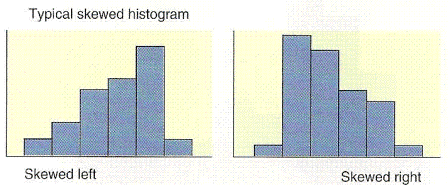
\includegraphics{img/skewed.png}
\end{figure}

Uniform distribution is a case when all the data values occur around the same
times, so we have no peaks, and such the variable has no mode. The tails of the
histogram are on its left or right side, where its extreme values are. A
histogram is left skewed if it has the left tail larger than the right, and
right skewed if the right tail  is larger than its left. 

\subsection{Empirical rule}

The empirical rule (also know as three $\sigma$ rule) states that for a normal
distribution $68\%$ of the data is within one standard deviation of the mean
value, $95\%$ is within two standard deviation, and $99.7\%$ is within three
standard deviation.

\section{Categorical variables}

Caterogical variables are not represented by numbers, so all of the earlier
statistics no longer make sense. What does make sense is the frequency of the
categories, which is graphically represented either by a barchart or a piechart.

Figure \ref{fig:category_representation} shows an example of this. In case of
barcharts we may choose to normalize the frequency, by dividing it with the
total number of observations.

\begin{figure}[htbp]
\label{fig:category_representation}
\caption{Skewed histograms}
\includegraphics{1/categorical_representation-categorical_representation}
\end{figure}
\chapter*{Releationships and data collections}
\addcontentsline{toc}{chapter}{Releationships and data collections}
\setcounter{section}{0}
\renewcommand*{\theHsection}{ch2.\the\value{section}}

\section{Relationship between quantitive and categorical variables}

Relationships are at the hearth of statistic. Let us consider an example. Let
there be the unit of observation the worlds countries. Now we define on this two
variables: a quantitive one -- the life expentancy, and a caterogical one -- in
which of the six world regions they fall into. Now we want to check for instance
if life expectancy in East Asia and Pacific tends to be larger than in the
Sub-Saharan Africe. 

One way of approach is to consider the median and mean per region, and to see
where this it's larger. However, this does not tells the whole story as the
highest in one of the regions can still be a lot higher than the lowest in
another region. Box plot is a graphical way to make the comparision.

Examining the relationship between a quantitative variable and a categorical
variable involves comparing the values of the quantitative variable among the
groups defined by the categorical variable. We need to:

\begin{enumerate}
  \item Examine the centre of the data in each group.
  \item Examine the spread of the data in each group.
  \item Examine the centre of the data in each group. 
\end{enumerate}

So create a boxplot (or summary) for each categorical observation and compare.

\subsection{In the R language}

In the R lanugage we can draw a new boxplot per category to make the
comparision. To separate categories we can use the \emph{split} function, and
finally use non-modified boxplots (\emph{range} is set to $0$) to draw them,
as seen on figure \ref{fig:boxplots}: 

\begin{minted}[numbersep=5pt]{r}
lifedata = read.table('LifeExpRegion.txt')
colnames(lifedata) = c('Country', 'LifeExp', 'Region')
attach(lifedata)
lifedata[Region=='EAP', ]
lifesplit = split(lifedata, Region)
lifeEAP = lifedata[Region=='EAP',]
lifeSSA = lifedata[Region == 'SSA', ]
boxplot(lifeEAP[,2], lifeSSA[,2], range=0, border=rainbow(2), 
        names=c('EAP', 'SSA'), main="Life Expectancies: Box Plot")
boxplot(LifeExp~Region, range=0, border=rainbow(6), 
               main='Life Expectancies: Box Plot (all 6 regions)')
\end{minted}

\begin{figure}[htbp]
\label{fig:boxplots}
\caption{Boxplots to compare quantitive and categorical variables}
\includegraphics{2/boxplots-boxplots}
\end{figure}

\section{Relationship between two categorical variables}

For instance let there be the two observations the gender of persons and their
body weight. One question we can ask is that are the same count of overweight
female as man?

\subsection{Distributions}

Distribution types are:

\begin{description}
  \item[joint distribution] of two categorical variables is the frequency or
  relative frequency of the observations considered together as a combination.
  The graphical approach is to use bar plots per combination, or aggregate these
  into a stacked bar plot.
  \item[marginal distribution] is the distribution of only one of the variables
  in a contingency table (so we take the total of the rows or of the columns in
  the table -- essentially its the distribution by only one of the variables).
  \item[marginal distribution] is the distribution of only one of the variables
  in a contingency table (so we take the total of the rows or of the columns in
  the table -- essentially its the distribution by only one of the variables).
  \item[conditional distribution] of a categorical variable is its distribution
  within a fixed value of a second variable. This distribution is normalized by
  the count of the fixed value. For graphical approach a stacked plot is used,
  by using the percentage values. Two variables in a contingency table
  indedependent if the conditional distribution of one variable is the same for
  all values of other variable.
 \end{description}

\begin{description}
  \item[Simpson's paradox] is when the conditional distributions within
  subgroups can differ from condition distributions for combined observations.
  The issue behind the paradox is that behind the two categorical variables ther
  is a third lurking variable which influences the study, like for a smoking
  study, to transform the age into age groups (if we study if the people die
  or not, having more old people in a group as observations may influence the
  result).
\end{description}
\subsection{Categorical values in R}

Categorical variables read into R are always sorted alphabetically, and
therefore any statistics about it will be displayed on that order. However,
sometimes there is a better order to this variables. In this case we can use the
\emph{factor} function and its \emph{levels} paramter to set a different order
for the categories: 

\begin{minted}[numbersep=5pt]{r}
allData <- read.table('SkeletonData.txt', header=TRUE) # dataset read 
attach(allData) # now we can use the column header names as variables
BMI = factor(BMI, levels = c('underweight', 'normal', 'overweight', 
                             'obese')) # reorder categories
\end{minted}

We can even give to the categories nicer names, as we do in the following
example for the sex categorical variable (which in the file is specified by the
values $1$ and $2$): 

\begin{minted}[numbersep=5pt]{r}
Sex = factor(Sex, levels=c('1', '2'), labels=c('Male', 'Female'))
\end{minted}

To find the number of items per category use the \emph{table} command. You can
divide tis with the number of observations to get the relative frequencies:

\begin{minted}[numbersep=5pt]{r}
relfreqBMI = table(BMI)/length(BMI)
\end{minted}

Which will result in the distribution of the data:

\begin{minted}[numbersep=5pt]{r}
BMI
underweight      normal  overweight       obese 
     0.1850      0.5625      0.2025      0.0500 
\end{minted}

We can even combine the relative and non relative values in a single table: 
\begin{minted}[numbersep=5pt]{r}
cbind(freqBMI, relfreqBMI)
\end{minted}

To get joint and the conditional distribution for two categorical variables we
need to use the \emph{CrossTable} function from the \emph{gmodels} library. 

\begin{minted}[numbersep=5pt]{r}
library(gmodels)
joint = CrossTable(BMI, Sex, prop.chisq=FALSE) 
  Cell Contents # legend for the table below
|-------------------------|
|                       N |
|           N / Row Total |
|           N / Col Total |
|         N / Table Total |
|-------------------------|
Total Observations in Table:  400  
             | Sex 
         BMI |      Male |    Female | Row Total | 
-------------|-----------|-----------|-----------|
 underweight |        46 |        28 |        74 | 
             |     0.622 |     0.378 |     0.185 | 
             |     0.164 |     0.235 |           | 
             |     0.115 |     0.070 |           | 
-------------|-----------|-----------|-----------|
      normal |       166 |        59 |       225 | 
             |     0.738 |     0.262 |     0.562 | 
             |     0.591 |     0.496 |           | 
             |     0.415 |     0.147 |           | 
-------------|-----------|-----------|-----------|
  overweight |        59 |        22 |        81 | 
             |     0.728 |     0.272 |     0.203 | 
             |     0.210 |     0.185 |           | 
             |     0.147 |     0.055 |           | 
-------------|-----------|-----------|-----------|
       obese |        10 |        10 |        20 | 
             |     0.500 |     0.500 |     0.050 | 
             |     0.036 |     0.084 |           | 
             |     0.025 |     0.025 |           | 
-------------|-----------|-----------|-----------|
Column Total |       281 |       119 |       400 | 
             |     0.703 |     0.297 |           | 
-------------|-----------|-----------|-----------|
\end{minted}

\begin{figure}[H]
\label{fig:two_categorical}
\caption{Relationship between two categorical variables}
\includegraphics[width=0.8\textwidth]{2/two_conditional-two_conditional}
\end{figure}

At this point the \texttt{joint} contains four tables: a contingency table
(frequencies -- \texttt{joint\$t}), two conditional distribution (one per point
of view -- sex \texttt{joint\$prop.col} or BMI \texttt{joint\$prop.row}), and
one displaying relative frequencies (joint distribution --
\texttt{joint\$prop.tbl}). We can use barplots to visualize this:

\begin{minted}[numbersep=5pt]{r}
layout(matrix(c(2,2,1,1), 2, 2, byrow = TRUE))
# side by side barplot
barplot(joint$t, beside=TRUE, col=rainbow(4), ylab='Frequency', 
                                              xlab='Sex')
# add legend information, 15 = plotting symbol, a little square
legend('topright', c('underweight', 'normal', 'overweight', 'obese'), 
                                            pch = 15, col=rainbow(4))
#stacked barplot
barplot(joint$prop.col, beside=FALSE, col=rainbow(4), 
                                      ylab='Frequency', xlab='Sex')
\end{minted}

as you can see it on figure \ref{fig:two_categorical}.

\section{Relationship between two quantitive variables}

One approach is to convert one (or both) of the quantitive variables into
categorical variable and then just use the already seen methods. One way to
create good groups is to use the quartile breakdown. However, this does not uses
the full information of the quantitive variables. 

One way to use it is to use a scatterplot (that is to use the quantitive
variable pairs as points in the space). On this we can use regression techniques
to fit a line on the points, effectively finding the relationship between the
variables (correlation means a rising line)

A numerical representation of this is the \emph{correlation}. Let there be two
variables indicated by the series $x_1, x_2, \ldots, x_n$ and $y_1, y_2, \ldots
y_n$, the correlation is calculated as:

\[ \mbox{correlation} = \frac{\sum_{i=1}^{n}\left( x_i-\bar{x}\right) \cdot
\left( y_i - \bar{y}\right)}{\sqrt{\sum_{i=1}^{n}\left( x_i-\bar{x}\right)^2
\cdot \sum_{i=1}^{n}\left( y_i - \bar{y}\right)^2}}
\]

Correlation values are between $[-1, 1]$, where $1$ is perfect match, and $-1$
is the perfect negative. If this is a positive value when one increases the
other tends to follow. However, note that this only captures the linear aspects
of the relationship.

\subsection{In the R lanuage}

For calculating the correlation we can use the \emph{cor} function.
 
\begin{minted}{r}
Countries = read.table('LifeGDPhiv.txt')
colnames(Countries) = c('Country', 'LifeExp', 'GDP', 'HIV')
attach(Countries)
plot(GDP, LifeExp, xlab='GDP(2000USD)', ylab='Life Expectancy (years)', 
     main='Scatterplot: Life Expectancy versus GDP per capita')
cor(GDP, LifeExp)
[1] 0.6350906
cor(LifeExp, GDP)
\end{minted}

\begin{figure}[htbp]
\label{fig:correlation}
\caption{Relationship between two quantitive variables}
\includegraphics[width=0.8\textwidth]{2/correlation-correlation}
\end{figure}

Figure \ref{fig:correlation} shows the information visually, when drawn on a
plot.

\section{Sampling}
The goal of the statistics is to make rational decision or conclusion based on
the incomplete information that we have in our data. This process is knows as
\emph{statistical inference}. The question is that if we see something in our
date (like a relationship between two variables) is it due to chance or a real
relationship? If it's not due to change then what broder conclusions we can
make, like generalize them to a larger group, or does it supports a theoretical
model? In this process the data collection has a major significance.

We collect data from the real world, however our scientific and
statistical models are part of a theoretical world. 

\begin{description}
  \item[population] the group we are interested in making conclusion about.
  \item[census] a collection of data on the entire population. This would be the
  best, however it's impractical due to time and cost effectiveness; or it's
  straight up impossible if by observing the item we would destroy it.
  Therefore, in practice we sample the population; and infer conclusions from
  the sample group.
  \item[statistic] is a value calculated from our observed data. It estimates a
  feature of the theoretical world.
  \item[paramter] is a feature of the theoretical world. Statistics are used to
  estimate their values. In order to get a good estimation our sampling needs
  to be \emph{representative}.
  \item[randomisation] is the key to select representative samples. This ensures
  that we do not over-- or under--sample any part of the population.  
\end{description}

Methods to make random sampling: 

\begin{description}
  \item[Simple Random Sampling -- SRS] Each possibly sample size of $n$ (the
  sample size) from the population is equally likely to be the sample that is
  choosen. A pratical example of this is taking out balls from a hat. 
  \item[Stratified sampling] Divide the population into non--overlapping
  subgroups called strata and choose a SRS within each subgroup. Provinces and
  states are a practical instances of stratas. This performs better when we may
  want to compare stratas, or can allow to better see traits if something is
  only characteristic to only some of the stratas (which otherwise would be
  hidden on the whole sample space).
  \item[Cluster sampling] Divide the population into non--overlapping subgroups
  called clusters, select clusters at random, and include all individual inside
  the cluster for sampling. It's good when it's easier to select groups instead
  of members; for example if we want to study students we may choose to select
  random schools and use students inside those as samples. This does requires
  that each cluster to be representative for the whole population.
\end{description}

There are also non--random sampling techniques:

\begin{description}
  \item[Systematic sampling] Select every $k$--th individual from a list of the
  population, where the position of the first person choosen is randomly
  selected from the first $k$ individuals. This will give a non--represenative
  sample if there is a structure to the list. This is fine if in the ordering of
  the population has no meaning.
  \item[Conveniance or Voluntar sampling] Use the first $n$ individuals that are
  available or the individuals who offer to participate. This is almost sure to
  give a non--representative sample which cannot be generalized to the
  population.
\end{description}

If the sample is not representative it can induce \emph{bias} into our results,
that is that it differs from its corresponding population in a systematic way.
Bias types are:

\begin{description}
  \item[Selection bias] occurs when the sample is selected in such a way that it
  systematically excludes or under--represents part of the population. For
  instance poll by using only land line phones (misses the cellular population).
  \item[Measurement or Response bias] occurs when the data are collected in such
  a way that it tend to result in observed values that are different from the
  actual value in some systematic way. In case of a poll this shows in terms of
  ill formed questions.
  \item[Nonresponse bias] occurs when responses are not obtained from all
  individuals selected for inclusion in a sample. An example of this is in a
  poll working parents tend to not respond, so their sampling will be under
  represented.
\end{description}

\section{Observational studies}

Whenever we want to compare the effect of variables on each other we need to
construct a study, for which sampling is really importat. Let us assume that we
have two (or more) groups,  and we want to compare a \emph{response variable}
(\emph{outcome}) between them. An \emph{explanatory variable} is a variable that
can be used to possibly explain the differences in the response variable between
groups (cause $\Rightarrow$ effect).

In the study we want to avoid \emph{confounding variables}, which differ between
groupsa and may effect the response variable so we can't tell what causes the
differences between groups. For instance if one were to study the effect of pot
on the IQ of the person, here a confounding variable is the social alternative
(which governs the IQ better, than the pot itself). 

Data collection methods include anecdotes (this are not representative),
observational studies and experiments. Experiments differ from observational
studie is the strength of the conclusion we can make, which is higher for the
experiment.

In observational studies we just observe existing characteristics of a subset of
individuals inside the population. The goal is to make conclusion about the
population based on the samples, or to conclude the relationship between groups
or variables in the sample. 

In this scenario the investigator has no control on which individual in which
group belongs or about any of their characteristic, as opposed to the experiment
where he can add some kind of intervention. 

The relationship between the outcome and the explanatory variable may be:

\begin{description}
  \item[causes] explanatory variable $\Rightarrow$ outcome (drinking coffe
  results in a longer life)
  \item[reverse causation] outcome $\Rightarrow$ explanatory variable (people
  with health issues avoid drinking coffe, though the longer life)
  \item[coincidence] pure chance
  \item[common cause] both of them are effected by another variable (who have
  diabiates drink less coffee, however due to their sickness have shroter life)
  \item[confounding variable] they vary with the explanatory variable. If one
  changes the other changes with it (smokers tend to drink more cofee, however
  this also effects the expected life outcome)
\end{description}

\emph{Lurking variables} are variables that are not considered in the analysis,
but may effect the natuer of relationship between the explenatory variable and
the outcome. This may be a confounding variable, or the source of the common
response , or another variable that, when considered, changes the nature of the
relationship.

\section{Experiments}

Are the golden standard. Allows for making conlusions. Again the response
variable (or also know as dependent variable -- how it depends from other
variables) is the outcome of interest, measured on each subject or entity
participating in the study (this may be quantitive or categorical). Explanatory
variable (predictor or independent variable) is a variable that we think might
help to explain the value of the response variable (can also be quantitive or
categorical).

Compared to the observation study now the researcher manipulates the explanatory
variables to see the effect of them on the outcome. Tipically a researcher has
finite time, and therefore he can study only a finit number of variable values,
and such the explanatory variable tends to be a categorical one, to which we can
also refer as a \emph{factor}. The values of the factor studied in the
experiment are its \emph{levels}.

A particular combination of values for the factors is called \emph{treatment}.
An \emph{experimental unit} is the smallest unit to which the treatment is
applied to. A treatment may not be applied to a single entity, like trying out a
new study method for a class results in a single experimental unit (a class)
instead of the count of the students inside the class.

\begin{description}
  \item[extraneous factors] are not of interest in the current study, but are
  thought to affect the reponse. They need to be controlled to avoid them
  effecting the outcome. For controlling we can: 
  \begin{itemize}
  \item Hold it constant. This limits the generilization of the study, however
  it also eliminates turning the extraneous variable into a confounding one.
  \item Use blocking, where block are groups of experimental units that are
  similar. All treatments are assigned to experimental units within each block.
  So for instance in a vaccine testing we create age groups, and each group will
  have have members getting any one of treatments, however the group as a hole,
  receives all the vaccines.
\end{itemize}
  However, this still does not solves the problem of extranous or unknown
  variables. To bypass this we need to use randomisation to assign experimental
  units to treatment groups.
\end{description}

Once we've eliminated other differences between the treatment groups, if the
response variable is different among the groups, the only explanation is the
treatment and casual conclusions can be made.

Fundamentals of experimental design:

\begin{enumerate}
  \item \emph{Control} the identified extraneous variables by blocking or
  holding them constant.
  \item \emph{Randomisation} -- is to randomly assign expermintal units
  to treatment groups.
  \item \emph{Replication} -- induce it. Not repeat the experiment, but to apply
  each treatment to more than one experimental unit. This allows to measure
  variability in the measurement of the response (which in turn also ensures
  that treatment groups are more comparable by extraneous factors, by having
  the oppurtunity of these to differ between groups).
\end{enumerate}

Experiments also have a control group. This is used to make comparisions with a
treatment of interest and either does not receives a treatment (what if the
study itself causes the change to occur) or receives the current standard
treatment. It's also refered to as the comparision group.

In conclusion we can say the randomised controlled experiments are needed to
establish casual conclusion. Another technique to reduce the potential of bias
is \emph{blinding}: 
\begin{enumerate}
  \item the experimental units are blinded, so they do not know which treatment
  they have received.
  \item the researcher is blinded if s/he does not know which treatment was
  given.
\end{enumerate}

Experimetns can be single--blinded (only one type of blinding was used) or
double--blind (if both types of blinding was used). You can also use the
\emph{placebo effect}. People often show change when participating in an
experiment wheater or not they receive a treatment. It's given to the control
group. A placebo is something that is identical to the treatment recevied by the
treatment groups, except that it contains no active ingridients.

\chapter*{Introduction to Probability}
\addcontentsline{toc}{chapter}{Introduction to Probability}
\setcounter{section}{0}
\renewcommand*{\theHsection}{ch3.\the\value{section}}

\section{The need for probability}

Up to this point we've seen and focused on how to handle data available to us.
Now it's time to see what the data in the real world corresponds in the
theoretical world. The data of the real world, that we usually end up having,
can be viewed as just a sampling of the theoretical world (which has an
infinit number of data points). Even if it really isn't any more data points in
the real world (so we have collected all the existing data points) we can still
pretend that there is and construct a theoretical model around it.

We usually try to draw inferences about our theoretical world by using the data
that we have, which represents the real world. Of course, the theoretical world
may differ from the real world and we'll be interested in studying the
relationship between two world. For instance let us consider a coin toss. In the
theoretical world we \emph{expect} to get $5$ heads out of ten tosses, yet if we
were to conduct a little experiment we may end up \emph{getting} $6$ heads out
of ten tosses.

In some cases (like tossing a bottle cap) we may not even have a theoretical
model, so the question arises that what we can conclude in this case? 

\section{Probability basics}

\begin{description}
  \item[Outcomes] are possible data that our experiment may result in. The set
  of all possible outcomes is the \emph{sample space} and it's noted as $S$.
  \item[Event] is any subset of the sample space.
  \item[Probability] -- each event has it's own probability to turn true, and
  for event $A$:
  \[
  0 \leq \mbox{P}(A) \leq 1 
  \]
  For example, the probability of some outcome is $1$, as we always end up
  having some result. The probability of the comploment event (meaning that
  event $A$ is not true) is:
 \[
  \mbox{P}(\bar{A}) = 1 - \mbox{P}(A)
 \] 
\end{description}

The term probability may have multiple interpretations: applies to a theoretical
world with a theoreticaal model where the probability for an event to occur is
P$(A)$; or we can look it as a long run, meaning that if we repeat the
experiment over and over again for a long time the occurance of event $A$ is
P$(A)$ fraction of all the events; another one is the subjective one: in my
opinion the chance that the event to occur is P$(A)$.

\section{Probability distributions}

For a coin or bear bottle fliping we use the binomial, not ass
B$(2,\frac{1}{2})$  distribution. If the exponential of the binomial is
one, we refer to it as te Bernoulli distribution: Bernoulli$(\frac{1}{2}) =
$B$(1, \frac{1}{2})$. The rolling of a dice is a discrete uniform
distribution.

\emph{Mean} is the expected value, what it equales ,,on average'' 

\[ \mbox{mean} = \mu = \sum_{x}x\mbox{P}(x)
\]

For instance in case of a rolling dice with six side:

\[
\mbox{mean} =
1\cdot\frac{1}{6}+2\cdot\frac{1}{6}+3\cdot\frac{1}{6}+4\cdot\frac{1}{6}+5\cdot\frac{1}{6}+6\cdot\frac{1}{6}=\frac{7}{2}=3.5
\]

For flipping two coins, with $Y$ being the total number of heads: 

\[
\mbox{mean}=E(Y)= 0\cdot\frac{1}{4}+1\cdot\frac{1}{2}+2\cdot\frac{1}{4} = 1
\]

\emph{Variance} in the theoretical world measures the spread of the values from
their mean value. The formula is:

\[
\mbox{variance} = \sum_{x} (x-\mu)^2\cdot\mbox{P}(x) 
\]

So for one coing flipping:

\[ \mbox{variance} =  \left(1-\frac{1}{2}\right)^2 +
\left(0-\frac{1}{2}\right)^2 + =  \frac{1}{4} \]

The \emph{standard deviation} is: 
\[ \mbox{SD} = \sqrt{\mbox{variance}} = \sqrt{\frac{1}{4}} = \frac{1}{2}
\]

The mean is linear, so any linear combination of two random variables may be
expressed with their means:

\[ \mbox{E}(aX+bY) = a\cdot\mbox{E}(X) + b\cdot\mbox{E}(Y)\]

For variance:



\begin{align*}
 \mbox{Var}(aX) &= a^2\cdot\mbox{Var}(X) \\ 
 \mbox{Var}(aX+b) &= a^2\cdot\mbox{Var}(X) \\
  \mbox{SD}(aX) &= |a|\cdot\mbox{SD}(X) 
\end{align*}

If $X$ and $Y$ are independent:
\[ \mbox{Var}(X+Y) = \mbox{Var}(X) + \mbox{Var}(Y) 
\]

Discrete random variables has a finit number of possible outcomes, and thus may
be enumerated in a form of a list. Continous random varaibles can take any value
inside an interval. An instance of this is the unifrom variable, for instance on
the interval from zero to one, meaning it's equally likeley to be any number
inside this interval. 

So for example P$(0 \leq X \leq 1) = 1$, and P$(0 \leq X \leq \frac{1}{3}) =
\frac{1}{3}$; generally speaking P$(a \leq X \leq b) = b - a$, if $0 \leq a \leq
b \leq 1$. This does mean that if $a=b$ the probability is zero, so it's easier
to think of continous probability as the area under the graph of the density
function. It's important that for any density function the total area of the
entire graph to be equal with $1$.

Uniform distributions are of a form of square function, however other functions
exist to like the exponential$(1)$ function has the form of: 

\[
 f(x) =
  \begin{cases}
   e^{-x} & \text{if } x > 0 \\
   0       & \text{if } x \leq 0
  \end{cases}
\]

The standard normal (Gaussian) distribution (bell--curve): 

\[ f(x)=\frac{1}{\sqrt{2\pi}} \cdot e ^{-\frac{x^2}{2}}\]

New bell--curves may be constructed by shifting the upper with $\mu$ (making it
the new center point) and stretching it by a factor of $\sigma$, and is noted as
Normal$(\mu, \sigma^2)$. If we have a random variable $X$ from this newly
constructed normal distribution we may transform it into a standard normal
distribution by: 

\[ 
Z = \frac{X - \mu}{\sigma} , \mbox{~ where $Z ${\raise.17ex\hbox{$\scriptstyle\mathtt{\sim}$}} Normal} (0,1). 
\]

For expected values and standard deviation now we use integals instead of sums,
for example the expected value of the uniform distribution between $0$ and $1$
is:

\[ \mbox{E}(X) = \int_{0}^{1}x\mbox{d}x = \frac{1}{2}  \]

with it's variance:

\[ \mbox{Var}(X) = \int_{0}^{1}\left(x - \frac{1}{2}\right)^2\mbox{d}x =
\frac{1}{12}
\]

For the exponential distribution it's expected value is:

\[ \mbox{E}(X) = \int_{0}^{\infty}x\cdot e^{-x}\mbox{d}x = 1  \]

with it's variance:

\[ \mbox{Var}(X) = \int_{0}^{\infty}\left(x - 1\right)^2\cdot e^{-x}\mbox{d}x =
1 \]

For the $X ${\raise.17ex\hbox{$\scriptstyle\mathtt{\sim}$}} Normal $(0,1)$: 

\[ \mbox{E}(X)  = \int_{-\infty}^{\infty}x \cdot \frac{1}{\sqrt{2\pi}}
\cdot e^{-\frac{x^2}{2}} \mbox{d}x = 0 
\]

\[ \mbox{Var}(X)  = \int_{-\infty}^{\infty} \left(x - 0\right)^2 \cdot
\frac{1}{\sqrt{2\pi}} \cdot e^{-\frac{x^2}{2}}\mbox{d}x = 1 
\]

And in case of $Y ${\raise.17ex\hbox{$\scriptstyle\mathtt{\sim}$}} Normal
$(\mu,\sigma^2)$ the mean is $\mu$, variance of $\sigma^2$ and standard
deviation of $\sigma$.

\section{Long running averages} 

What happens if you repeat an experiment lots of times and you look at the
average value you get. For example if you start flipping a coin a lot of times
and you look at the fraction of times you get head, you expect that the more you
do it, the more this comes closer to half. If you were to draw the probabilities
of the coin flip on a graph, you'd observe that the shape starts to resemble the
density function for the normal distribution. The same is the case for dice
rolling at looking the average of the rolled numbers.

\emph{The Law of Large Numbers} states that if an experiment is repeated over
and over, then the average result will converge to the experiment's expected value.

\emph{The Central Limit Theorem} states that if an experiment is repeated over
and over, then the probabilities for the average result will converge to a
Normal--distribution.

Suppose that an experiment is repeated over and over, with outcomes: $X_1, X_2,
$ $~\ldots$ and suppose each mean is E$(X_i) = m$, and each variance is is
Var$(X_i)=v$. Now let $\bar{X} = \frac{X_1 + X_2 +\ldots + X_n}{n}$ be the
average outcome. In this case we can say that:

\[ \mbox{E}(\bar{X}) = \frac{\mbox{E}(X_1) + \mbox{E}(X_2) + \ldots +
\mbox{E}(X_n)}{n} = \frac{nm}{n} = m,\]

\[ \mbox{Var}(\bar{X}) = \frac{\mbox{Var}(X_1) + \mbox{Var}(X_2) + \ldots +
\mbox{Var}(X_n)}{n} = \frac{nv}{n^2} = \frac{v}{n},\]

so we can conclude as n rises to infinity the variance (uncerteinty) becomes
smaller and smaller, tending to zero; with this the standard deviation too.

The centreal limit theorem also is responsible for the emparical rule; the
percentages are true for the graph of the normal distribution. In conclusion we
can say that all that is some kind of average, or is made up of lots and lots of
small contributions usually has a normal distribution behind it.

\section{Sampling distribution}

From the real world we collect samples, which can be considered as part of the
theoretical worlds population. We have scientific and statistical models in the
theoretical world which have parameters of features that we do not know. We use
the science of statistics to estimate them.

Let there be $p$ our parameter of interest, what we are observing, and let it
denote the number of heads of a coin flip sequence. From the real world (data)
we get some result. With this we can esitmate the parameter as:

 \[ \hat{p} = \frac{\mbox{numbers of heads observed}}{\mbox{number of coin
 flips}}\].
 
 The observed value of an estimator varies from sample of data to sample of
 data. The variability of this is called the \emph{sampling variability}. The
 probability distributions of the possible value of an estimator is its sampling
 distribution.
 
 A statistic used to estimate a paramters is \emph{unbiased} if the expected
 value of its sampling distribution is equal to the value of the parameter being
 estimated (the sampling probability is the same as the theoretical
 probability). How close the distribution of the sampling gets to the parameter
 dependes on the varince of the sampling distribution. This decreases with the
 number of samples, so the more data we have the closer we get to the
 theoretical word.
 
 Following the central limit theorem for large $n$ the sampling distribution for
 a Bernoulli event (happens or not, with probability $p$) is N$\left( p,
 \frac{p(1-p)}{n}\right)$ (sampling distribution of $\hat{p}$).
 
 If we take a normal distribution as a sample distribution with a normal
 distribution theoretical model we can calculate the expected value of the
 theoretical model as the average of the sample we have, and the standard
 deviation of the theoretical model decreases with the number of data compared
 to the standard deviation of the sampling distribution
 ($\frac{\sigma}{\sqrt{n}}$). The sampling distribution of $\bar{X}$ is N$\left(
 \mu, \frac{\sigma^2}{n}\right)$.
 
 For calculating the variance dividing with $n-1$ is important to make the
 estimator unbiased, while dividing with $n$ will result in a bias estimator.
 

\chapter*{Confidence interval}

\addcontentsline{toc}{chapter}{Confidence interval}
\setcounter{section}{0}
\renewcommand*{\theHsection}{ch4.\the\value{section}}

We observe the real world in order to understand the theoretical world; for this
we'll use the scientific and statistical models divised in the theoretical world
and use data from from the real world to estimate the paramters from the model.
We do this in hope that what conclusions we can make from our models will also
hold in the real world.


Now let us imagine the experiment of tossing a fair coin ten times. This
experiment has a binomial distribution with probability $\frac{1}{2}$, however
when amassing data from the real world we will not always get this proportion,
due to the sampling having its own distribution: for example extreme events
(like getting ten heads) are very unlikely, however getting half or close to
half of them heads is likely to happen. The question arrises where do we draw
the line, what are the values well likely to get most of the time?

Sometimes we will not have a model for our events: like in the case of flipping
a beer cap. If we were to perform a single experiment and get $m$ one side
out of $n$ events we can ask: was this a likely outcome? $m$ may be a sample of
any sample distribution (with its own parameters). For instance for the beer cap
let $n=1000$ and $m=576$. Our statistical model is binomial with a $1000$
samples, however we have no idea what's the probability of the model. 

An estimation is $\hat{p}=\frac{n}{m}=\frac{576}{1000}=0.576$. This may be a
good estimate, however it may be some other number, and so we ask what elso
could $p$ be? That is what is an interval that based on our existing experiments
the probability of getting one side of the beer cap could be? We refer to this
as the \emph{confidence interval}. 

The following methods are suppose that our data was taken in a form of simple
random sampling, and that our variables are independent; something that
statistical inference requires, otherwise we may need more complicated model.

So in conclusionwe can say that the goal of statistical inference is to draw
conclusions about a population parameter based on the data in a sample (and
statistics calculated from the data). A goal of statistical inference is to
identify a range of plausible values for a population parameter. A goal of
statistical inference is to identify a range of plausible values for a
population parameter. Inferential procedures can be used on data that are
collected from a random sample from a population.


\section{Confidence intervals with proportions}

Let us follow the example of the bottle cap. We are searching for the real $p$
with the given estiamte $\hat{p}$. The expected value of $\hat{p}$ is
$\mbox{E}(\hat{p})=p$ the variance is $\mbox{Var}(\hat{p}) =
\frac{p(1-p)}{n}=\frac{p(1-p)}{1000}$. Now according to the center limit theorem
because $p$ is the addition of lots and lots of small flips, it approximately
follows the normal distribution; that is $\hat{p} \approx
\mbox{Normal}\left(p, \frac{p(1-p)}{1000}\right)$. Now by performing a
reorganization: 

\[ \frac{\hat{p}-p}{\sqrt{p\cdot\frac{1-p}{n}}} \approx \mbox{Normal}(0,1) \]

Now for a normal distribution (and according to the empirical rule) the area
between $[-1.96, 1.96]$ covers $95\%$ of the area, so most likely our sample is
from this interval. In mathematical formula:


\[ \mbox{P} \left( \left| \frac{\hat{p}-p}{\sqrt{p\cdot\frac{1-p}{n}}} \right| >
1.96\right) = 0.05 = 5\%
\]

By writing up the reverse, and expanding we can conclude that, with
$z_{\frac{\alpha}{2}} = 1.96$:

\[ \mbox{P} \left( \underbrace{\hat{p} - \overbrace{z_{\frac{\alpha}{2}}\sqrt{p
\cdot \frac{1-p}{n}}}^{\mbox{margin of error}}}_{\mbox{lower limit}} \leq p \leq
\underbrace{\hat{p} + z_{\frac{\alpha}{2}}\sqrt{p \cdot
\frac{1-p}{n}}}_{\mbox{upper limit}} \right) = 95\%
\]
This means that we are $95\%$ confident that the value of $p$ is between is
lower and upper limit. Now the true value of $p$ is not random, however
$\hat{p}$ is as we took a random sample. Now the problem with this formula is
that while we do know $\hat{p},~p$ is unknown. One solution is to make
$\hat{p}=p$; or to make $p=\frac{1}{2}$ because that's the worst case, the
widest interval we can get.

For a given confidence interval $[a,b]$ the margin of error may be calculated
as:

\begin{align*}
a &= \hat{p} - \mbox{margin of error} \\
  b &= \hat{p} - \mbox{margin of error} \\ 
  \mbox{margin of error} &= \frac{b-a}{2}
\end{align*} 

Now modifying the area under the normal distribution that we take we can get
different confidence intervals for different probabilities. Now if you specify a
bigger confidence value, like $99\%$ you'll get a widder confidence interval.
It's up to you the trade off you are willing to accept.

Now assume you want to achive an $\alpha$ probability that you're wrong. In
this instance taken the graph of the normal distribution you want to find
$z_{\frac{\alpha}{2}}$ (y axis) such that the area remaining at each and is only
$\frac{\alpha}{2}$. In this case the area between intervals
$-z_{\frac{\alpha}{2}}$ to $z_{\frac{\alpha}{2}}$ is $1-\alpha$, which we are
looking over, as now we're missing $\alpha$ of the full area.

\section{Sample size for estimating a proportion}

Now in order to get a proportion the size of the sample has a major impact.
Let's see how we can determinate the sample size we need to find a given
proportion. We do not want to go overboard with this as we may just waste
resources or induce unrequired effort to collect it. We assume that data was
collected with simple random sampling from a population.

So a margin of error is: 

\[ \mbox{margin of error} = z_{\frac{\alpha}{2}}\sqrt{p \cdot
\frac{1-p}{n}}\]

For isntance, if our confidence interval is $95\%$, then 
$\frac{\alpha}{2}=\frac{1-0.95}{2}=0.025$, and we want a margin of error of
$\beta=0.03$. The question is what $n$ should be? For $95\%$ our normal quantile
is $1.96$. So:

\[ 0.03 = 1.96\sqrt{p \cdot
\frac{1-p}{n}}\]
 
 But we do not know what $p$ will be. To bypass this we plan for the worst case
 scenario, the expression $p\cdot(1-p)$ has its maximum at $p=\frac{1}{2}$,
 which also give our maximal margin of error for a given $n$. Now we resolve the
 equation:
 
 \[ n=\left( \frac{1.96 \cdot \frac{1}{2}}{0.03} \right)^2 = 1067 \]

Confidence intervals are about our confidence in the procedure to give us
correct results -- $95\%$ confidence intervals should contain the population
parameter $p 95\%$ of the time. If simple random samples are repeatedly taken
from the population, due to the randomness of the sampling process the observed
proportion of $\hat{p}$ will change from sample to sample and so will the
confidence interval constructed around $\hat{p}$. Of these confidence intervals,
$95\%$ will include the true population proportion $p$.

Note that $p$ is a population parameter and is therefore not a random variable.
For any interval, $p$ is either contained in the interval or not. Different
margin of error will result in different number of events required, however the
sample size increases quadratically as the margin of error decreases linearly.

\section{Confidence intervals for means}

In this case the data is not a categorical one, is instead a continous variable.
In this case the expected value is $\mu = \bar{X}$, and this is also our
estimation. The variance is equal to $\frac{\sigma^2}{n}$. Again if the data is
made up of the sum of bunch of small measurements, we can assume according
to the center limit theorem that $\bar{X} \approx \mbox{Normal}\left(\mu,
\frac{\sigma^2}{n}\right).$ Again we reduce this to the standard normal
distribution to get:

\[ \frac{\bar{X}-\mu}{\sqrt{\frac{\sigma^2}{n}}}  \approx \mbox{Normal}
\left( 0, 1\right)
\]

Now the problem now is that we do not know the value of $\sigma$. What would be
a good estimation for this? One solution is to use the standard deviation of $X$
(calculated with dividing with $n-1$), noted as $s$. However, while
$\mbox{E}(s^2)=\sigma^2$, substituting this into upper formula does not gives a
normal distribution; instead we'll have a $t$ distribution with $n-1$ degrees of
freedom:


\[ \frac{\bar{X}-\mu}{\sqrt{\frac{s^2}{n}}}  \approx t_{n-1}
\]

The $t$ distribution is similar to the normal one, however not quite there.
Increasing the degree of freedom reduces the difference between these two.
With this the $z_{\frac{\alpha}{2}}$ changes also, so you'll need to use a table
to get the correct number for a given number of freedom (which is $n-1$, where $n$ is
the sample size). The marginal error may be calculated as:

\[ \mbox{marginal error}= z_{\frac{\alpha}{2}} \cdot \sqrt{\frac{s^2}{n}} \]

We can use this to calculate the true mean from a sample mean. That is with a
given confidence we can say that our true mean is somewhere inside the
calculated confidence interval, which depends from the sample mean with the
calculated marginal error.

\section{Robustness for confidence intervals}

To use these methods many conditions must be satisfied, and an important part of
the statistical inference is to determine if these hold. Here are what we need
to make sure that they are true:

\begin{enumerate}
  \item the $n$ observations are independent,
  \item $n$ needs to be large enough, so that the central limit theorem may kick
  in and $\hat{p}$ to have a normal distribution, 
\end{enumerate}

For extreme theoretical $p$ values larger counts of samples are required to
achieve the same confidence interval. For instance in case of a coin flip if $p$
is $\frac{1}{2}$ a hundred samples may be enough for the central limit theorem
to kick in and achive a $95\%$ confidence. However, if $p=0.01$ we may need
$1000$ samples for the same confidence. An explanation for this is that the
normal distribution is a continous model, and we are using it to estimate 
discrete values.

In order for the confidence interval procedure for the true proportion to
provide reliable results, the total number of subjects surveyed should be large.
If the true population proportion is close to $0.5$ a sample of $100$ may be
adequate. However, if the true population proportion is closer to $0$ or $1$ a
larger sample is required.

Increasing the sample size will not eliminate non-response bias. In the presence
of non-response bias, the confidence interval may not cover the true population
parameter at the specified level of confidence, regardless of the sample size.
An assumption for the construction of confidence intervals is that respondents
are selected independently.

In case of means the conditions are:

\begin{enumerate}
  \item the $n$ observations are independent
  \item $n$ needs to be large enough so that $\bar{X}$ is approximatly normally
  distributed.
\end{enumerate}

The $t$ distribution works extremly well with even a low number of samples ($n
=10$) if the theoretical model is a normal or skewed normal one. For this to not
be true we need some really extreme distribution, like most of the time on one
end, but has some chance for an outlier value. However, in these cases by just
increasing the mean with a constant multiplier (like to $40$) may already result
in a $90\%$ confidence value. 

Nevertheless, we also need to consider if estimating the mean is a meaningful
thing to do. Remeber that the mean is not a robust measurement, because it's
effected by outliers, something that is true for the distribution too.

A method for constructing a confidence interval is robust if the resulting
confidence intervals include the theoretical paramter approximately the
percentage of time claimed by the confidence level, even if the necessary
condition for the confidence interval isn't satisfied.

\chapter*{Statistical Tests of Significance}

\addcontentsline{toc}{chapter}{Statistical Tests of Significance}
\setcounter{section}{0}
\renewcommand*{\theHsection}{ch5.\the\value{section}}

Suppose that we observe the difference between two groups, the question now is
that is the difference significant or not? It's the answer to the question could
that be just due to change; or it says something else about the nature of the
date. 

Once we collect data from the real world, we already saw how we can construct
models that about the theoretical world. Based on the models we can make some
conclusions about our situation in the real world. For instance, if we collect
samples from a population by examining the sample set we may draw conclusions
about the entire population. The test of significance is about is our
observation is only due to chance or it may even shed light on some wrongful
asssumptions about the theoretical world. 

For example, assume we have the life expectancies of the countries in East--Asia
and the Sub--Saharan Africa. We can see that on average this is smallre for the
African region, however is this just an effect of the natural variability of
data, or holds something more to it. To observer this we construct a theoretical
model that assumes that there is no difference between the groups. We are either
searching for proof of this or some contradiction, based on our data amassed.

\section{The structure of the statistical test}

\subsection{Assumption}

Statistical math is like proof by contradiction in math. We start out by
assuming something. Then we observe the date, do some calculations and
eventually end up with a contradiction; such we conclude that there must be
something wrong about our assumption, our theoretical model. Of course, we are
in the domain of statistic something is wrong is actually meaning that the model
is unlikely to hold true in the real world.

\emph{Tests} are used to answer questions about the theoretical world, and the
goal is to check if the data collected provides enough evidence that the
theoretical model holds in the real world. Statistical tests are also called
hypotetical test, or tests of significance. The first step of any statistical
test is to formulate the hypothesis: is the flipping of a beer cap like a coint
flipp? Afterwards you need to state an alternative to the hypothesis.

A real world analogy is a court case. We start out from the assumption that
everyone is innocent until proven otherwise. In statistics this corresponds to
the \emph{null hypothesis}  ($H_0$ -- pronounced as ,,H-naught''). This states
that nothing is happening; that is that there is no relationship, no difference.
We assume that this is true and check weather our date support it or contradicit
it.

The \emph{alternative hypothesis} corresponds to the guilty alternative in the
court case, and it corresponds usually to what the reaseach tries, wants to
show (noted as $H_a$ or $H_1$ or $H_A$). We may conclude that this is true if we
can proove that $H_0$ is false, in other words rule out that any difference
between $H_A$ or $H_0$ is due to chance.

Alternatives may be \emph{one--} or \emph{two--sided}. One sided is the case of
the beer cap, our assumption holds true or not; while a two sided example is the
effect of plastical surgery on the perceived age of a person, here our null
hypothesis is that there is no change, and we have two alternative, they either
look younger or older.

\subsection{The evidence}
In the court to proove our claim we'll need evidence. In statistics the
evidences are proovided by the data we have. In order to make it useful we have
to summarize our data into a \emph{test statistic}; whcih is a numeric
representation of our data. This is always formulated such that it's assumed
that the null hypothesis holds. In case of the plastic surgery we summarize data
assuming that the perceived age difference is zero, to support our null
hypothesis.

\subsection{Delibiration}
Once the evidences are presented the judge/jury delibirates if beyond a
reasonable doubt the null hypothesis holds or not. In statistics the tool of
delibiration is the \emph{p--value}. This transforms a test statistics into a
probability scale; a number between zero and one that quantifies how strong the
evidence is against the null hypothesis.

At this point we ask, if the $H_0$ holds how likely would it be to observe a
test statistic of this magnitude or large just by chance? The numerical answer
to this question is the p--value. The smaller this is the stronger evidance it
is against the null hyptothesis. However, it is not an a measurement to tell you
how likely it is that the $H_0$ is true.

$H_0$ is or it is not true, however it's not a random variable, because it's
either true or not true, no randomness involved. The p--value just tells you how
unlikely the test statistic is if the $H_0$ were to be true.

\subsection{The verdict}

The fourth final step is the verdict. Not strong enough evidance corresponds to
a high p--value. With this we conclude that the data is consistent with the null
hypothesis. However we haven't yet prooved that it's true, although we cannot
reject it either. A small p--value consist of sufficient evidence against $H_0$,
and we may reject it in favour of $H_A$. In this case the result is
statistically significant.

It remains one question to be answered: how small is small? There's no clear
rules on this, hower it's a good practice that $p<0.001$ is very strong, $0.001
< p < 0.01$ is strong, $0.01 < p < 0.05$ is moderate, while $0.05 < p < 0.1$ is
weak. A larger p--value holds no strength against $H_0$. The cut off value you'l
want to use is context based, with smaller values if that would lead to
inconveniances.

If there is not enough evidence to reject the null hypothesis, the conclusion of
the statistical test is that the data are consistent with the null hypothesis.
The null hypothesis cannot be proven true. For example, imagine an experiment
where a coin is flipped $100$ times and we observe $52$ heads. The null
hypothesis may be that the coin is fair and the probability of heads on any flip
is $0.5$.
The alternative hypothesis would be that the probability of heads on any one
flip is not $0.5$.

The observed data show $52$ heads out of $100$ flips and that is not convincing
evidence to reject the null hypothesis. These data are consistent with the null
hypothesis $p=0.5$ but would also be consistent with a null hypothesis that the
probability of heads is $0.5000001$ or $0.501$ or $0.52$ or many other values.

\section{Hypothesis Testing for Proportions}

We'll use the following situation to visualize: there has been a poll with
$n=1,046$ people from which $42\%$ said that they support the mayor. So the true
support for the mayor is unknown ($p$), however the estimated is $\hat{p}=0.42$.
What we want to know if the true support is less than $50\%$:

\begin{itemize}
  \item $H_0: p = 0.5$
  \item $H_A: p < 0.5$
  \item Question: can we reject $H_0$?
\end{itemize}

We want to compute the p--value. We start out from our theoretical model, that:

\[ \mbox{test statistic} = \frac{\hat{p}-p}{\sqrt{p\cdot\frac{1-p}{n}}} \approx
\mbox{Normal}(0,1)
\]

Now by doing the substitution for the known values:

\[ \frac{\hat{p}-p}{\sqrt{\frac{1}{2}\cdot\frac{1-\frac{1}{2}}{1046}}} \approx
\mbox{Normal}(0,1)
\]
 
Now assumign $H_0$ is true $\hat{p}-p=0.42-0.5=-0.08$. So our p--value is the
probability of observing this value under the $H_0$ hypothesis:

\[ \mbox{P}(\hat{p}-p < -0.08) = \mbox{P} \left(
\frac{\hat{p}-p}{\sqrt{\frac{1}{2}\cdot\frac{1-\frac{1}{2}}{1046}}} \leq 
\frac{-0.08}{\sqrt{\frac{1}{2}\cdot\frac{1-\frac{1}{2}}{1046}}} \right)
\approx \mbox{P}\left( \mbox{Normal} \left( 0,1\right) \leq -5.17 \right)
\approx \frac{1}{9,000,000}
\]

This is an extremly small value, which means that our evidence against the null
hypothesis is strong, therefore we may reject it, and conclude that the mayors
support is less than $50\%$. If we were to put in a lower number into the
equation we may check just how small the mayors support it is. For example in
case of $44\%$ we'l get a numbe of $0.0968$, which means that under the null
hypothesis we have a $\approx 10\%$ chance to sample this, and that's not a
strong evidence aginst $H_0$.

If we have a two sided hypothesis then instead of P($Z \geq$  test statistic) we
can say that P($|Z| \geq$  test statistic)=P($Z \geq$  test statistic) $+$
P($Z <-$  test statistic), which in case of symmetric distributions
translates to $2\cdot$P($Z \geq$  test statistic).

\section{Hypothesis Testing for Means}

As test case for this we'll use the plastic surgery data, where we were
interested just how much younger are people perceived after the surgery. The
question is that all patiance will look younger or have we been just lucky? We
had $n=60$ persons in the survey, where after the surgery people looked younger
on average with $\bar{X}=7.177$ years with a standard deviation of $2.948$
years.

So formulating the problem we can say that in the real world we have the true
mean (noted as $\mu$), with an estimated mean of $\hat{\mu}=\bar{X}=7.177$. Our
null hypothesis is that people do not look younger, $H_0:~\mu=0$; with hour
alternative hypothesis is that $H_A:~\mu>0$. Now we saw previously that:

\[ \frac{\bar{X}-\mu}{\sqrt{\frac{s^2}{n}}}  \approx t_{n-1}
\]

We also know from our observation that $\bar{X}-\mu=7.177-0=7.177$. The p--value
is the probability of observing such an extreme value given that $H_0$ is true.

\[ \mbox{P} \left( \bar{X} - \mu \geq 7.177\right) = 
\mbox{P} \left( \frac{\bar{X}-\mu}{\sqrt{\frac{s^2}{n}}} \geq
\frac{7.177}{\sqrt{\frac{s^2}{n}}}  \right)
\]
Now we got something for what we know its distribution, it's:

\[ \mbox{P} \left( t_{59} \geq \frac{7.177}{\sqrt{\frac{(2.948)^2}{60}}}\right)
= \mbox{P} \left( t_{59} \geq 18.86 \right) = \frac{1}{10^{26}}
\]

Which is really small, and such we can reject the null hypothesis.

\section{Powerand Type I and Type II Errors}

We start out from the null and the alternative hypothesis. We then calculate
thep p--value representing the probability of observing the value of the test
statistic given that $H_0$ is true. Small p--values are evidence against the
$H_0$.

\begin{description}
  \item[significance level] of a test gives a cut--off value for how small is
  small for a p--value. We note it with: $\alpha$. This gives a definition for
  the reasonable doubt part of the method. It shows how the testing would
  perform in repeated sampling. If we collect test statistics again and again
  sometime we'll get weird data. So for a significance level of $1\%$ in case of
  $100$ we'll draw the wrong conclusion in one case (reject $H_0$). Setting it
  to small however would result that you never reject $H_0$. 
  \item[power] of the test is the probability of making a correct decision (by
  rejecting the null hypothesis) when the null hypothesis is false. Higher power
  tests are better at detecting false $H_0$. To do this you'll need to:
  \begin{itemize}
  \item power increases the further our alternative hypothesis is from the null
  hypothesis (however in practice this is rarely in our control), 
  \item $\alpha$ is increased then less evidence is required from the data in
  order to reject the null hypothesis; therefore for increased $\alpha$, even if
  the null hypothesis is the correct model for the data, it is more likely that the null
  hypothesis will be rejected;
  \item less variability increases,
  \item increasing the sample sizea also helps.
\end{itemize}
 To determine the sample size needed for the a study for which the goal is to
 get a significant result from a test, set $\alpha$ and the desired power,
 decide on an alternative value that is practically interesting, estimate
 $\sigma$, and calculate the sample size required to to give the desired power.
 \item[type I error] is incorrectly rejecting the null hypothesis, as we got
 data that seemed unlikely with the data we got. For a fixed significance level
 $\alpha$ the probability of this happening is $\alpha$.
 \item[type II error] is incorrectly not rejecting the null hypothesis, the
 probability of this is $\beta = 1 - \mbox{power}$. This usually happens because
 we do not have enough power due to small data size.
\end{description}

Generally we would like to decrease both types of errors, which can be done by
increasing the sample size (as having more evidence in a trial). It's context
dependent which of the errors are more important.

\section{Potential pitfalls to look out for}

Do not miss interpret p--values. It does not tell you how likely it is that
$H_0$ is true. It tells you how likely the observed data would be if $H_0$
holds. The p--value is a measure of significance. Therefore report it whenever
you make conclusions.

Data collection matters! Testing cannot correct flaws in the design of the data
collection: not randomly choosing samples, lack of control, lack of randomising
in assigning treatments. All these would lead to bias, confounding and variables
inable to make conclusions.

Always use two--sided test, unless you're sure apriori that one direction is of
\emph{no} interest.

Statistical significance is not the same as practical significance. Just because
it's significant statistically it does not mean that it's also meaningful
practicaly. For example let us suppose we want to measure the tempatures of
people. For this we'll use a huge sample size, compared to the small already
existing one.

The increased sample size means that even a small difference from the expected
mean temperature under the null hypothesis may be declared statistically significant.
For example we could demonstrate that a difference of $0.005$ degrees would be
significant statistically. While this is very precise, there is not much
practical significance especially because most commercial thermometers do not
measure the temperature with such a high precision.

A large p--value does not necessarily means that the null hypothesis is true.
There may not be enough power to reject it. Small p--values may happen due:

\begin{itemize}
  \item chance,
  \item data collection issues (lack of randomization),
  \item violation of the conditions required by the testing procedure used,
  \item or because the null hypothesis is false.
\end{itemize}

If multiple tests are caried out, some are likely to be significant by chance
alone. So we need to be suspicious when you see few significant results when
many tests have been caried out; such as significant results on a few subgroups
of data.

Test results are not reliable if the statement of the hypothesis are suggested
by the data. This is called \emph{data snopping}. Generally the primary
hypothesis should be stated before any data is collected. Seeing some relation
in the data and testing for it is not good, as in this the p--value does not
says anything.

The tests presented here require:

\begin{itemize}
  \item independent observations
  \item the sampling distributions of the estimators to be (approximately)
  normally distributed.
\end{itemize}

Any statistical test is deemed robust if it is not dependent on this
requirements. While the independent is hard to go around, the sampling
distribution is not. A good example of this is that although we have discrete
values, for instance in case of a coin flip, we can still use the test method
although the norma distribution is continous.

Start with explanatory analysis using plots and summary statistics. If you can't
visualize it you may wonder if its important even if from a statistical point of
view it's significant. It is not appropriate to extrapolate the results from a
regression model since the relationship between the response and dependent
variable may change.

\chapter*{Tests, Confidence Intervals, and Comparing Two Samples}

\addcontentsline{toc}{chapter}{Tests, Confidence Intervals, and Comparing Two Samples}
\setcounter{section}{0}
\renewcommand*{\theHsection}{ch6.\the\value{section}}

One may ask what relation there is between the confidence intervals (what's a
range of plasauble values for a quantity) and the hypothesis testing (provides a
\emph{yes} por \emph{no} answer indicating if we can reject the null hypothesis
or not)? There exist one relation between two--sided confidence intervals and
two--sided hypothesis test. To illustrate this let us consider the bottle cap
tossing experiment: 

\begin{description}
  \item[hypothesis test] the null hypothesis is $H_0: p=0.5,$ versus the
  alternative hypothesis $H_A: p \neq 0.5$ (two--sided). We have $n=1000$
  observations, which gives an estimated probability $\hat{p}-0.576$, so
  $|\hat{p}-0.5|=0.076$. This results in a p--value $=P(|\hat{p}-0.5| \geq
  0.076) \approx P(|\mbox{Normal}(0,1)| \geq 4.81) = \frac{1}{663,000} <
  0.05 (\mbox{typical significance level})$, so we reject the null hypothesis.
  
  \item[confidence interval] the $95\%$ confidence interval is $\hat{p} \pm
  1.96 \sqrt{\frac{p(1-p)}{n}}$, where $1.96$ is the critical value
  taken from the standad normal distribution (multiplied by the standard
  deviation) $= [0.545, 0.607]$, which misses the $0.5$.
\end{description}

So we got somehow the same result by using two different methods. This is not
chance, this happens generaly a lot. Thus it can be said that we reject the null
hypothesis exactly when the confidence interval misses the expected average
value.

If one considers a single sample, and considers a two sided test versus a two
sided confidence interval then it's exactly the same thing at whatever
significance level $\alpha$, to reject the null hypothesis or the corresponding
confidence interval does not includes the null hypothesis value. 

The range of plasauble values  will include a certain particular value if and
only if that particular value would have been rejected by the corresponding
hypothesis test.


For a sampled data, as the confidence level is increased, the width of the
confidence interval also increases. For example for a reported p-value of
$0.02$, and $\mu=97$, all confidence intervals with a confidence level equal to
or greater than $98\%$ will contain $97$ as a plausible value for $\mu$. All
confidence intervals with confidence level less than $98\%$ will not contain
$97$ as a plausible value for $\mu$.

\section{Matched pairs}

There are situations when we no longer need to observe a single variable.
Sometimes there are two different measurements/groups, and tell if these two
differ. This section will look into methods to do just this. 

As case study let us take the antrepology example, that is estimating the age
of death for persons taken from observing bones. Our observation values are the
errors of the methods from the actual ages of death. The DiGangi method tends to
underestimate the age of death, as for more than $75\%$ of measurements the
error is negative. This is on average $\approx -14$. 

The Suchey--Brooks method uses different bone to estimate, though may offer
different values. The mean for this is $\approx -7$, so this too underestimates.
However, these numbers are taken from just a handful ($n=400$) samples, so the
question rises are these two methods actually different?

\emph{Matched pairs} are useful when we want to compare two conditional
variables, and we are able to compare them on the same or two very similar
observational or experimental units (same subject, or twins/siblings). For
example age estimates on the same skeletons with different methods, or testing
the same subjects under two different condition (pre and post course).

However, the matching can also be time, like when we want to compare two
branches of a business, and we compare sales for the same week. The
\emph{crossover study} is when we have two treatments, and we compare their
outcome by giving to each experimental unit first one treatment, and then the
other one.

This means that we do not need to randomize experimental units, as
everyone will get all treatments. However, the order each experimental unit
receives the treatment is randomized, to avoid cases that the effect of a later
treatment is affected by an earlier treatment. Therefore, the variation in the
comparision does not include the variation among observational or experimental
units, resuling in a greater precision in the estimate of the difference between
the treatments or conditions being compared.

Measurements on a matched pair are not independent, resulting in the better
precision, however the analysis must reflect the pairing. The general approach
is to treat each pair as a separate observation, and then they will all be
independent, because each sceletong is independent. A way to do this is to
take the difference between the two methods as a new observed variable.

A practical problem is that what we do for experimental units for which one of
the measurements is missing, not available? An easy solution is to just ignore
these. Now let the difference be noted as $d$. We state our null hypothesis that
there is not difference between the methods, that is $H_0: \mu_d=0$ versus
$H_a: \mu_d \neq 0$. From our dat we know what $\bar{X}_d=6.854, s_d = 11.056$,
and $n=398$. We can formulate the test statistic as:

\[ \frac{\bar{X}_d - 0}{\frac{s_d}{\sqrt{n}}} = \frac{6.854 -
0}{\frac{11.056}{\sqrt{398}}} \doteq 12.37 
\]

If the null hypothesis is true this test statistic should be a value from a
t--distribution with a $398$ degree of freedom. The degree is quite high, so the
t--distribution is very close to the standard normal distribution. In case of a
standard normal distribution $99.7\%$ of data is within three standard
deviation, that is between $[-3,3]$. So a value greater than $12.37$ or smaller
than $-12.37$ is very unlikely. If one were to calculate a p--value it would
contain $29$ zeros after the decimal point.

We can conclude that we have an extremely strong evidence that the null
hypothesis is not true. So the two methods results differ, in giving the mean of
the age error estimation.

To construct the confidence interval with a $95\%$ confidence, for a data set
with $398$ observation we need to take a t--distribution with $397$ degree of
freedom, for whoose area is $0.95$, thush resulting in the critical values of
$-1.96$ and $+1.96$: 

\[ \bar{X}_d \pm \mbox{critical value} \cdot 
\frac{s_d}{\sqrt{n}} = 6.8554 \pm 1.966 \cdot \frac{11.056}{\sqrt{398}} \doteq
[5.76, 7.94 ] \]

Therefore, we estimate the difference between the two methods is low as $5.76$
and high as $7.94$. Because the hypothesis test held a strong evidence that the
mean of the difference is not zero, this confidence interval does not contains
the zero value.

It's important to understand that multiple measurements on the same subject are
not independent since two measurements within one subject are more likely to be
similar than two measurements on different subjects. For example, two math test
scores for the same student will likely be more similar than math test scores
chosen from two random students.

\section{Comparing two proportions}

In this case again we have two different conditional variables, however now they
are no longer result of observing the same experimental unit, they are
independent:

\begin{itemize}
  \item sample size $n_1$, success fraction $\hat{p}_1$,
  \item sample size $n_2$, success fraction $\hat{p}_2$.
\end{itemize}

What we are interested is $\hat{p}_1 -\hat{p}_2$, which has a mean of $p_1-p_2$,
with a variance calculated as Var($\hat{p}_1-\hat{p}_2)=\mbox{Var}(\hat{p}_1) +
(-1)^2 \cdot
\mbox{Var}(\hat{p}_2)=p_1\cdot\frac{1-p_1}{n_1}+p_2\cdot\frac{1-p_2}{n_2}$. If
the two variables are reasonably large sized then the central limit theorem
still applies and we can say that $\hat{p}_1 - \hat{p}_2 \approx \mbox{Normal}$
$\left(p_1-p_2, \frac{p_1(1-p_1)}{n_1}+\frac{p_2(1-p_2)}{n_2}\right)$, that is
it approximatly follows the normal distribution. 

Again we transform this to a standard normal distribution:

\[ \mbox{Normal}(0,1) \approx \frac{(\hat{p}_1 - \hat{p}_2) - (p_1 -
p_2)}{\sqrt{\frac{p_1(1-p_1)}{n_1}+\frac{p_2(1-p_2)}{n_2}}}
\]

Now the problem is that the value of $p_1$ and $p_2$ are unknown. For confidence
intervals one can approximate $p_1$ with $\hat{p}_1$, and $p_2$ with $\hat{p}_2$
respectively. At this moment for a $95\%$ confidence interval we can calculate:

\[ \hat{p_1} - \hat{p_2} \pm 1.96
\sqrt{\frac{\hat{p}_1(1-\hat{p}_1)}{n_1}+\frac{\hat{p}_2(1-\hat{p}_2)}{n_2}} \]

From the resulting confidence interval one may conclude if the difference
changed, either in a positive or a negative direction.

In case of a hypothesis test the same logic applies, let there be $H_0: p_1 =
p_2$ versus $H_A: p_1 \neq p_2$, knowing that $ \mbox{Normal}(0,1) \approx
\frac{(\hat{p}_1 - \hat{p}_2) - (p_1 -
p_2)}{\sqrt{\frac{p_1(1-p_1)}{n_1}+\frac{p_2(1-p_2)}{n_2}}}$. Now under $H_0$,
we assume that $p_1=p_2$, so we approximate both of the $p_1$ and $p_2$ with 
$\hat{p}=\frac{n_1\cdot \hat{p_1} + n_2 \cdot \hat{p_2}}{n_1 + n_2}$, also
refered as the pooled estimate. Therefore, we can say that: 

\[ \mbox{Normal}(0,1) \approx \frac{(\hat{p}_1 - \hat{p}_2) - (p_1 -
p_2)}{\sqrt{\hat{p}\cdot(1-\hat{p})\cdot\left(\frac{1}{n_1} +
\frac{1}{n_2}\right)}}
\]

This may be used to compute p--value: $P(|\hat{p_1}-\hat{p_2}| \geq \hat{p})$.

\section{Comparing means}

To compare the difference between two independent variables true means with a
sample size of $n_1$ and $n_2$, means of $\hat{X}_1, \hat{X}_2$ and variance of
$s_1^2$ and $s_2^2$ one can reuse the following fact:

\[
\frac{(\hat{X}_1-\hat{X}_2)-(\mu_1-\mu_2)}{\sqrt{\frac{s_1^2}{n_1}+\frac{s_1^2}{n_1}}}
\approx t_{df}
\]

The relation approximatly hold however the degree of freedom is given by the
equation:

\[ df = \frac{\left(\frac{s_1^2 }{n_1} + \frac{s_2^2 }{n_2} \right)^2} {
\frac{\left(\frac{s_1^2 }{n_1}\right)^2}{n_1-1} + \frac{\left(\frac{s_2^2
}{n_2}\right)^2}{n_2-1} } 
\]

Now the confidence interval for $\mu_1-\mu_2$ may be calculated as:

\[ \hat{X}_1 - \hat{X}_2 \pm T_{\frac{\alpha}{2}, df} \sqrt{\frac{s_1^2}{n_1}
+ \frac{s_2^2}{n_2}}
\]

For hypothesis test, the null hypothesis test is that the difference is zero.
Now we reusze the uppper approximation to compute p--values. Under the null
hypothesis we cannot pool together the means, like we did for proportions unless
we also assume that the two series have the same variance. The p--value may be
found as:

\[ \approx P \left( |t_{df}| \geq
\frac{|\bar{X}_1-\bar{X}_2|}{\sqrt{\frac{s_1^2}{n_1} + \frac{s_2^2}{n_2}}} \right) 
\] where the degree of freedom is calculated with the upper formula.

If the variances are equal we can pool them, as under $H_0$ we have the same
mean and variance, by using for both $s_1^2$ and $s_2^2$ the pooled variance:
$s^2 = \frac{(n_1-1)\cdot s_1^2 + (n_2-1)\cdot s_2^2}{(n_1-1)+
(n_2-1)}$. Under this assumption to calculation of degree of freedom simplifies
to the forumla $df = (n_1-1)+(n_2-1) = n_1 - n_2 - 2$. Now, note that the
sample variance does not need to be the same, what needs to be equal is the true
variance of the samples ($\sigma_1^2$ and $\sigma_2^2$).
\chapter*{Linear Regression}

\addcontentsline{toc}{chapter}{Linear Regression}
\setcounter{section}{0}
\renewcommand*{\theHsection}{ch7.\the\value{section}}

Linear regression (or lines of best fit) may be used to understand linear
relationship between data. For two variables the dependent (response) variable
is noted as $Y$, while the independent (explanatory, predictor) variable is
noted as $X$. The equation of a line looks like $y=b_0+b_1 \cdot x$. Now we try to
come up for values for $b_0$ and $b_1$ which are the best they can be to
describe the data as well as possible.

For this one can assume that a given point ($x_i$) the $y_i$ may be calculates
as $b_0+b_1 \cdot x_i$. However, the actual value we have is $y_i$ making the
difference between them $y_i-(b_0+b_1 \cdot x_i)$ (residiual). Now we
don't want them to be just small, because then they may turn negative, a nice way of
doing this is to make the $(y_i-b_0-b_1 \cdot x_i)^2$ as small as possible.


So for a whole dataset we will try to minimize the sum of squares:

\[ SS = \sum_{i=1}^n (y_i-b_0-b_1 \cdot x_i)^2 \]

This may be achieved by making:

\[ \frac{\partial}{\partial b_0}SS = \frac{\partial}{\partial b_1} SS = 0 \]

resulting in the formulas:

\begin{align*}
b_0 &= \frac{1}{n} \left( \sum_{i=1}^{n} y _i - b_1 \sum_{i=1}^{n} x_i \right)
\\
b_1 &= \frac{n \sum_{i=1}^{n} x_i \cdot y_i - \sum_{i=1}^{n} x_i 
\cdot \sum_{i=1}^{n} y_i}{n \cdot \sum_{i=1}^{n} x_i^2 - \left(\sum_{i=1}^{n}
x_i \right)^2}
\end{align*}

$b_0$ is also called the intercept and $b_1$ is the slope. A slope ($b_0$) of
$\alpha$ means that when the explanatory variable increases by $1$ the response
variable increases by $\alpha$. The intercept variable is what the response
variable would be in case of an explanatory variable with zero value. It is how
much we have to shift the line in order to get the line of best fit.

Regression is not symmetric, that is if you swap the explanatory and the
predictor variable the slope value will not turn out to be the inverse.

\section{Regression Coefficients, Residuals and Variances}

The intercept coefficient may be reformulated as:

\[b_0 = \frac{1}{n} \left( \sum_{i=1}^{n} y _i - b_1 \sum_{i=1}^{n} x_i \right)
 = \bar{y} - b_1 \cdot \bar{x} \] so, the regression line $y$ value
 corresponding to $x_i$ is:
 
 \[ b_0+b_1\cdot x_i = (\bar{y} - b_1 \cdot \bar{x}) + b_1 \cdot x_i =
 \underbrace{\bar{y}}_{\mbox{start from mean}} + \overbrace{b_1 \cdot (x_i -
 \bar{x})}^{\parbox[t]{5cm}{shift by how far we are \\ multiplied by the slope}}
 \] 
So, if $x_i=\bar{x}$, then we end up with $\bar{y}$, meaning that the point
$(\bar{x}, \bar{y})$ is on the line.

In case of the slope coefficient we can also reformulate, first by dividing top
and bottom with $n^2$:

\[ b_1 = \frac{\frac{1}{n} \sum_{i=1}^{n} x_i \cdot y_i -
\left( \frac{1}{n} \sum_{i=1}^{n} x_i \right) \cdot \left(
\frac{1}{n} \sum_{i=1}^{n} y_i \right)}{\frac{1}{n} \cdot \sum_{i=1}^{n} x_i^2 -
\left(\frac{1}{n} \sum_{i=1}^{n} x_i \right)^2} \] and then rewrite it by adding
in $\bar{x}$ and $\bar{y}$:
\[ b_1 = \frac{\frac{1}{n} \sum_{i=1}^{n} x_i \cdot y_i -
\bar{x} \cdot \bar{y}}{\frac{1}{n} \cdot \sum_{i=1}^{n} x_i^2 -
\left(\bar{x} \right)^2}\] which can be rewritten to: 
\[ \frac{\frac{1}{n} \sum_{i=1}^{n} (x_i - \bar{x})(y_i - \bar{y})
}{\frac{1}{n}\sum_{i=1}^{n}\left( x_i - \bar{x} \right)^2} = \frac{
\sum_{i=1}^{n} (x_i - \bar{x})(y_i - \bar{y}) }{\sum_{i=1}^{n}\left(
x_i - \bar{x} \right)^2} = b_1 \].

Now we'll reformulate this to: 

\[ \frac{\sum_{i=1}^{n}(x_i - \bar{x})(y_i - \bar{y})}{\sqrt{\sum_{i=1}^{n}(x_i
- \bar{x})^2 \sum_{i=1}^{n}(y_i -
\bar{y})^2}} \times \frac{\sqrt{\sum_{i=1}^{n}(y_i - \bar{y})^2}}
{\sqrt{\sum_{i=1}^{n}(x_i - \bar{x})^2}} = b_1 = R \times \frac{s_y}{s_x}\],
where $R$ is the correlation, and $s_x$ is the sample standard deviation for $x$
with $s_y$ the sample standard deviation for $y$.

The residiual is the difference between the actual and the predicted value, for
the $i^{\mbox{th}}$ it may be calculated $e_i=y_i-b_0-b_1 x_i$, the mean
$\bar{e}$ is $0$, as sometime we overshoot, sometime we underestimate however on
average we get it just right. 

\begin{align*}
\mbox{Var} (e)&=\frac{1}{n-1}\sum_{i=1}^{n} (e_i -
\bar{e})^2 \\ 
&= s_y^2 + (R \frac{s_y}{s_x})^2 s_x^2 - 2 R \frac{s_y}{s_x}
\frac{1}{n-1} \sum_{i=1}^{n} (x_i - \bar{x})(y_i - \bar{y}) \\
&= s_y^2 (1-R^2)\\
&= \mbox{Var}(y)(1-R^2)
\end{align*} 

So we can conclude that regression multiplies the variance by $(1-R^2)$, that is
the regression line ''reduces'' or ''removes'' a fraction of $R^2$ of the
variance of the $Y$. That is the linear relationship explains $R^2$ fraction of
the variation. The $R^2$ is the coefficient of determination and show how much
ofthe data is explained by the linear relationship. If this is zero
(correlation) it means that it explains nothing, while an $R^2=1$ explains
everything, once you have $x_i$ you already know $y_i$. 


\section{Regression Inference and Limitations}

How much certainty is there on the values introduced in the earlier section?
Maybe those values are right for the data world, however the true values (for
the theoretical world) there may be slight variations. For the theoretical world
we note the ''true'' slope as $\beta_1$. How close is the data world slope
($b_1$) to $\beta_1$. It's true that the distribution of
$\frac{b_1-\beta_1}{SE(b_1)} ${\raise.17ex\hbox{$\scriptstyle\sim$}} $ t_{n-2}$,
that is it follows a t--distribution with $n-2$ degree of freedom (one degree
loose for the slope, and one extra for the intersect). 

The $SE(b_1)$ is the standard error involved given by the formula:

\[ SE(b_1) = \frac{\sqrt{\sum_{i=1}^n e_i^2}}{\sqrt{(n-2) \sum_{i=1}^n (x_i -
\bar{x})^2 }} \mbox{ where } e_i = y_i -b_0 - b_1 x_i
\]

Now, we can use this t--distribution to calculate (carry out) for the slope the: 

\begin{description}
  \item[confidence interval] of $(1-\alpha)$ for $\beta_1$ is $b_1 \pm
t_{\frac{\alpha}{2}, n-2} SE(b_1)$
	\item[hypothesis test] we start out again from
the t--distribution written up, use the null hypothesis that $H_0: \beta_1 = 0$
and the alternative that $H_A: \beta_1 \neq 0$.

For the p--value we'll use the formula: P$(|b_1-\beta_1| \geq b_1)$ under the
null hypothesis, which can be rewritten to P$\left(|t_{n-2}| \geq
\frac{b_1}{SE(b_1)}\right)$. If the p--value is small we reject the null
hypothesis, that is that there is no linear relationship. Note, that this does
not implies causation, because that would require a randomised experiment. It
only concludes that there is some kind of relationship.
\end{description}
 
As for limitations we can say that linear regression can only tell about linear
relationship. It tells nothing for other relationships like (like quadratic).
Moreover there are cases when even if we have perfect numbers, we  still cannot
tell if the numbers tell, what they mean. Therefore, it's important to draw the
data, and visualize it. Linear regression is not robust to the presence of
outliers. Therefore, it's important whenever analyzing data that these may skew
the results.

The value of the slope $b_1$ should be interpreted relative to its standard
error, $SE(b_1)$. For example, imagine a regression of weight on height for
college students. We know that there is a strong positive association between these two
quantities so it would not be surprising to be able to reject the null
hypothesis that $\beta_1=0$. This will be true regardless of the units of
measurement of either variable. 

Note that the estimates of the slope and the standard error will change
depending on the units of measurement. If weights are measured in kilograms but
height in millimetres, $b_1$ and $SE(b_1)$ will be large values. If weights are
measured in kilograms but height in kilometres, $b_1$ and $SE(b_1)$ will be
extremely small values but there will still be strong evidence of a linear
relationship between height and weight.

\section{Residual Analysis and Transformations}

The question will cover that are the two variables relationship well described
by a linear relationship? For this we'll study the residual values (the
difference between where a predicted value should be accoring to the linear
regression, and where it actually is). In case of linear relationship the
residiuals should not have any trend, there should be equally spread out in the
space if one were to plot them.

If the residual plot shows a trend it means that the linear relationship does
not tells the whole story. For such cases, one could do a transformation to
eliminate such. A such transformation is the logarithmic transformation, with a
base $10$ for example.

Now note that the transformation on the plot also transforms the slope values,
so the increase/decrease is no longer linear.
\chapter*{The Process of Statistical Inquiry}

\addcontentsline{toc}{chapter}{The Process of Statistical Inquiry}
\setcounter{section}{0}
\renewcommand*{\theHsection}{ch8.\the\value{section}}

In the process of statistical inquiry it's essential to understand the  context:
which data, how collected, on whom and for what? We should always keep this in
mind while analysing the numbers. The sequence of steps in a study are:

\begin{description}
  \item[formulate] a clear (perhaps single) focused research question. Sometimes
  research questions may evolve, and in this case it's important and required to
  confirm them with future studies and new data. 
  
  We make statistical studies for two reasons: build a model for making
  \emph{predict}ions or to enhance \emph{understanding of the relationships}
  between variables (where they occur and their nature). In case of the later to
  specify a single research question, one primary purpose (that is to study one
  outcome variable).
  
  In case of data mining or machine learning the goal is to build predictive
  models from large amounts of data, often without an explicit research
  question. Data mining work tends to be more algorithmic than based on
  probability models and statistical properties.
  \item[design and implement] a study to acquire data that are relevant to the
  research question.
  \item[examine] the data for problems.
  \item[carry out preliminary and then formal] analyses
  \item[iterpret and present] the results
\end{description}

\section{Formulate}

A clearly stated purpose makes the results of any study more compelling. It is
always the case that performing multiple tests increases the chance of making a
type I error, as would be the case if we were to perform a statistical test
repeatedly for each of multiple outcome variables.

Sometimes investigators specify multiple outcomes, and then insist on a smaller
significance level for their tests in order to avoid type I errors. But this
reduces power compared to a larger significance level for one outcome, and thus
increases the chance of making a type II error. 

Be cautious of studies that investigate many outcomes, and emphasize only the
statistically significant findings. Non-significant findings are interesting
too. And type I errors are not interesting. When planning a study, a clear
question, with a clear difference of interest, with a desired significance level
and power, are necessary to calculate the required sample size for the study.

In this quest we first must formulate our primary question. Then follow this up
with some potential secondary question. For each of this question we must
formulate a variable that measures accuratly and obiectivly the answer to those
question. Then we need to separate the explanatory and the outcome variables.

\section{Design}

We want to design and implement a study to acquire data that are relevant to the
research questions. To do this we need to be able to generalise conclusions to a
population of interest, avoid any systematic error (biases) in both the
measurements and conclusions, reduce the non systematic error caused by the
natural variability for more precises estimates and power in our conclusions,
and ensure that the sample is appropiate to have enough power to make
conclusions (and to avoid making unnecessary measurements).

The first question is what kind of study to carry out:

\begin{description}
  \item[anecdotal] Anecdotal evidence doesn't lead to conclusions that can be
  generalized beyond the current observations.
  \item[sample survey] (poll) requires to be able to make measurements only with
  questions 
  \item[observational study] while allows to conduct the observations in the
  experimental units natural enviroment, it does not allow making casual
  conclusions. However, it carries the risk of common cause and confounding
  variables.
  \item[experiment] if controlled and ramomized allow us to make full inference.
  The principles of an experimental design is control (what we can -- hold
  some variables constant, use of blocking -- choose subjects appropiately
  with inclusion and exclusion criterias), randomisatio (selection of
  experimental units and assigment of treatments)n and replication (number of
  subjects to acquire statistically significant results).
\end{description}

\section{First look at the data}

At this step we need to identify problems in the data and also some of the
preliminary analisys. Look for obvious errors and identify features (outliers,
skew, etcetera) that may effect the choice of analysis. 

For categorical variables use barplots and pie charts. For quantative variable
use boxplots and histograms. Missing values, if they are completly random, will
not introduce bias into the results. However, if they missing is due to some
causual effect then those values are informatitive and their lack may
potentially lead to bias results.

\section{Formal analysis}

Formal and preleminary analysis are an interative process. What you learn from
formal analisys may cause to look at the data in new ways, which then will lead
to new formal analysis.

Although the t--test is a very robust measurement, it does not works in every
situation (non normal distribution), so it's important to take a look at the
date first prior to applying it. The removal (or lack) of outliers will give
more power for our statistical tests (resulting in lower p--values).

The central limit theorem needs large sample sizes when making comparisions with
proportions that are close to zero. There are cases that were not covered inside
this course: 

\begin{description}
  \item[analysis of variance] to compare more than two means
  \item[longitudinal analysis] analyse not just the difference (and start plus
  end point) between two values, but the way those two variables got there. 
  \item[control the chance] of making type I errors in multiple tests.n
\end{description}

\end{document}